We received 2 simulations from Floren: one with $\tilde{N}=12$ points and one with $\tilde{N}=24$. In this section, we compare the results from the algorithms for both $N=8$ and $N=20$. In order to isolate the \textit{spatial} error, we compare our solution with a strong stability preserving third order Runge Kutta (SSP RK3) time integrator to the solution Floren sent with the lowest timestep. The SSP RK3 solutions are accurate to 10 or more digits, as verified by refining the timestep by a factor of 2 and comparing solutions (for $N=8$, $\Delta t =10^{-6}$, for $N=20$, $\Delta t =10^{-7}$). The ``exact'' solution is defined to be the one Floren sent with $\tilde{N}=24$ and smallest timestep $\Delta t=10^{-6}$. 

Fig.\ \ref{fig:L2} shows the $L^2$ errors of 3 simulations: both ours and Floren's when $N=8, \tilde{N}=12$, and ours when $N=20$. Our algorithm gives 3 digits of \textit{absolute} accuracy in the fiber position for $N=8$ and 4 digits for $N=20$. 

Fig.\ \ref{fig:poser12} gives the absolute error at $t=0.01$ as a function of the arclength position along the fiber for $N=8, 20$ for both Floren's and our simulation. We observe about 3 digits of absolute accuracy for $N=8$ and 4 digits for $N=20$. In general, the relative accuracy is 10 times the absolute accuracy (i.e. 10 times worse), since the points move approximately $\mathcal{O}(0.1)$ throughout the simulation. 

Note also that the absolute accuracy of Floren's solution for $\tilde{N}=12$ is 1-2 digits. This translates to a relative accuracy of 0-1 digit. That is, there is an error of 10-100\% in the motion of the points (especially near to the boundaries). \textbf{Thus the spatial error for our discretization is $10^{-3}$ for $N=8$ points, but for Floren's it is $10^{-2}$, or even larger near the boundary. Thus, at least for this spatial discretization, our algorithm is more accurate. }


\begin{figure}
\centering 
\subfigure[$L^2$ norm]{
\label{fig:L2}
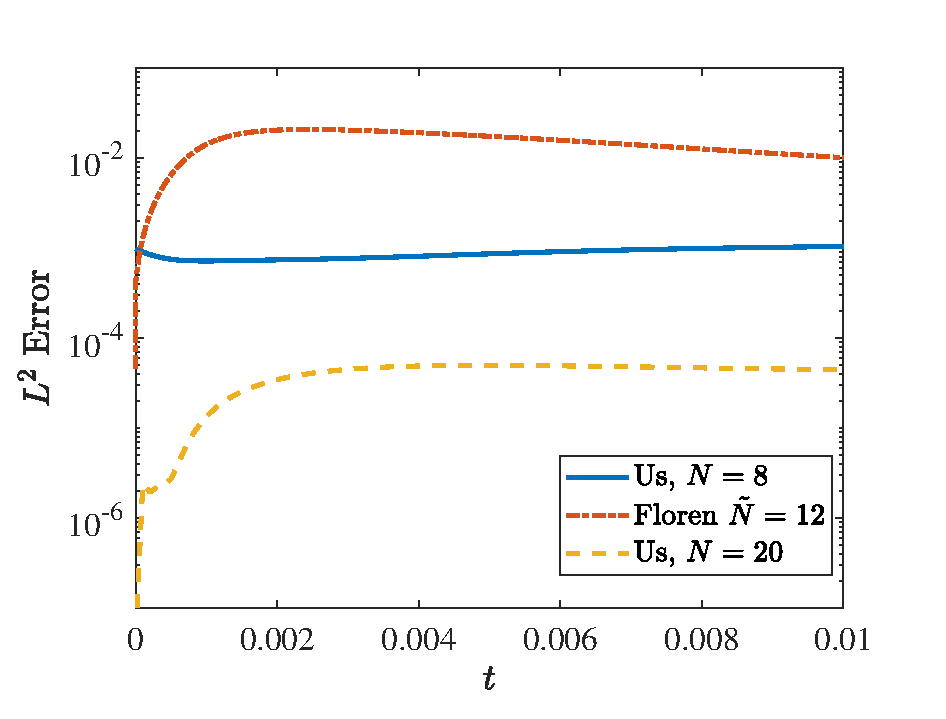
\includegraphics[width=70mm]{SimonsL2Compare.eps}}
\subfigure[Error by position]{
\label{fig:poser12}
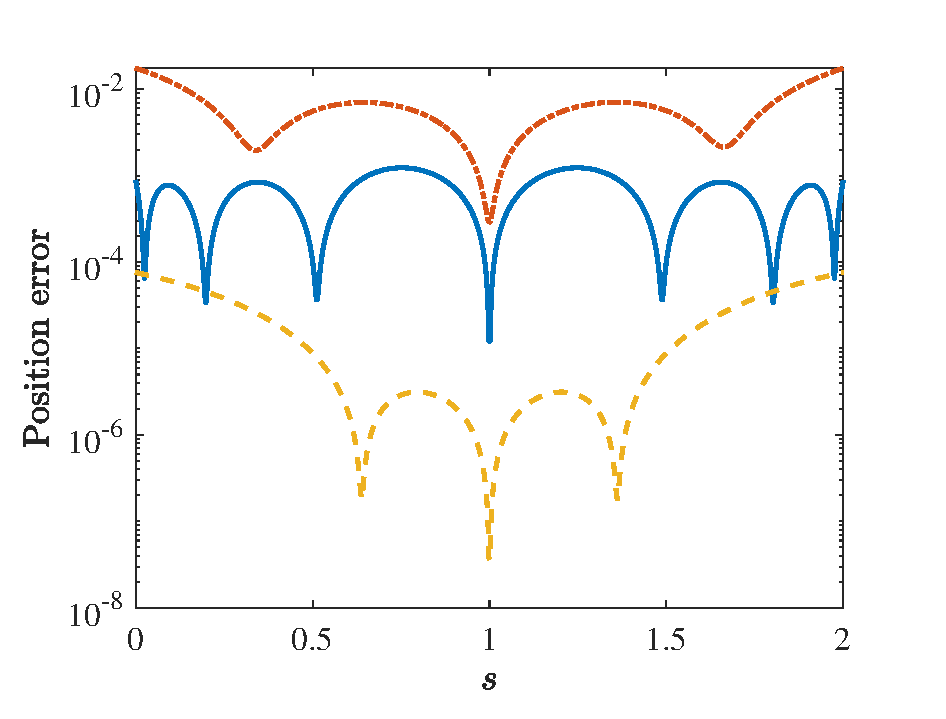
\includegraphics[width=70mm]{ErrorbyPosition.eps}}
\caption{Errors from 3D fiber simulation. (a) $L^2$ norm over time for $N=8$ (solid blue), $N=20$ (dashed yellow). The norm is defined in Eq.\ \eqref{eq:Errort}. The $L^2$ error in Floren's data for $\tilde{N}=12$ is shown as a dashed-dotted red line. (b) The absolute error in the positions along the fiber (at $t=0.01$) for $N=8$, $N=20$ (same color scheme as (a)). The spatial errors are isolated by using an SSP RK3 scheme for our method and using the lowest timestep provided for Floren's method.} 
\end{figure}

\subsubsection{Inextensibility}
\label{sec:inext}
We consider how inextensible the fiber truly is for $t > 0$. In \cite{ts04}, a penalty parameter $\beta$ is added to the line tension equation to preserve inextensibility. In this section, we compare this formulation to our formulation, where the inextensibility is constrained by the allowed fiber motion, Eq.\ \eqref{eq:du}. 

To measure the inextensibility error, we take the fiber positions $\bm{X}$, upsample them to a fine grid, apply the spectral differentiation matrix on the fine grid to compute $\bm{X}_s$, and then measure the maximum difference of its norm from 1 along the fiber at every timestep. Fig.\ \ref{fig:inext} shows the results for simulations with negligible temporal error. While Floren's code with the penalty parameter (solid lines) generally performs better, we are still able to enforce inextensibility to 2  digits for $N=8$ and 6 digits for $N=20$.

\begin{figure}
\centering
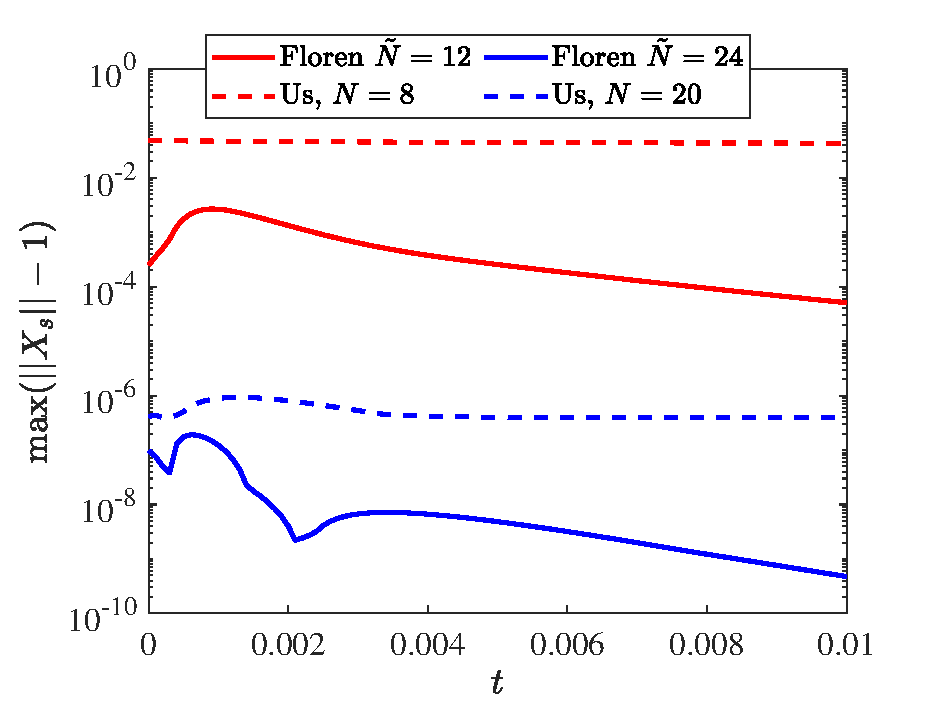
\includegraphics[width=70mm]{Inextensibility.eps}
\caption{Error in enforcing the inextensibility constraint, $\textrm{max}\left|\norm{\bm{X}_s}-1\right|$ for $N=8$, $\tilde{N}=12$ (red lines) and $N=20$, $\tilde{N}=24$ (blue lines). Solid lines show the results from Floren's code with the penalty parameter, while dashed lines show the results for our algorithm with constrained motion. }
\label{fig:inext}
\end{figure}

\subsubsection{Boundary conditions}
One of the features of our method is that boundary conditions are enforced in a weak sense with rectangular matrices (as opposed to a strong sense with square matrices). To verify this, we consider the fiber configuration $\bm{X}$ at time $t$. We perform differentiation on the type 1 grid and upsample the result to a type 2 grid with 1000 points (this is numerically preferable to upsampling and then differentiating). We consider the norms $\norm{\bm{X}_{ss}(s=0)}$ and $\norm{\bm{X}_{sss}(s=0)}$ of the upsampled derivative (these quantities are the same at $s=L$ by symmetry and should both be zero). 

Fig.\ \ref{fig:BCs} shows the error in the boundary conditions as a function of time for $N=8, 12, 16$ and $20$. As in Section \ref{sec:inext}, the configurations are generated using RK3 temporal integration with $\Delta t =10^{-6}$ to isolate the spatial error. For both $\bm{X}_{ss}$ and $\bm{X}_{sss}$, we observe spectral convergence. 

\begin{figure}
\centering 
\subfigure[$\norm{\bm{X}_{ss}(s=0)}$]{
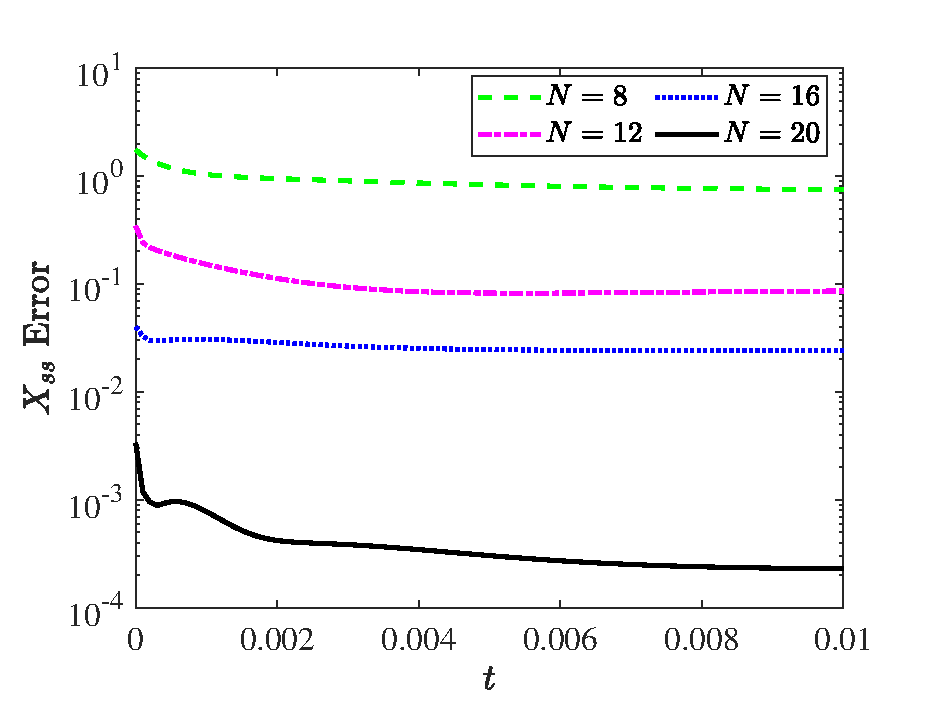
\includegraphics[width=70mm]{BCErrorXss.eps}}
\subfigure[$\norm{\bm{X}_{sss}(s=0)}$]{
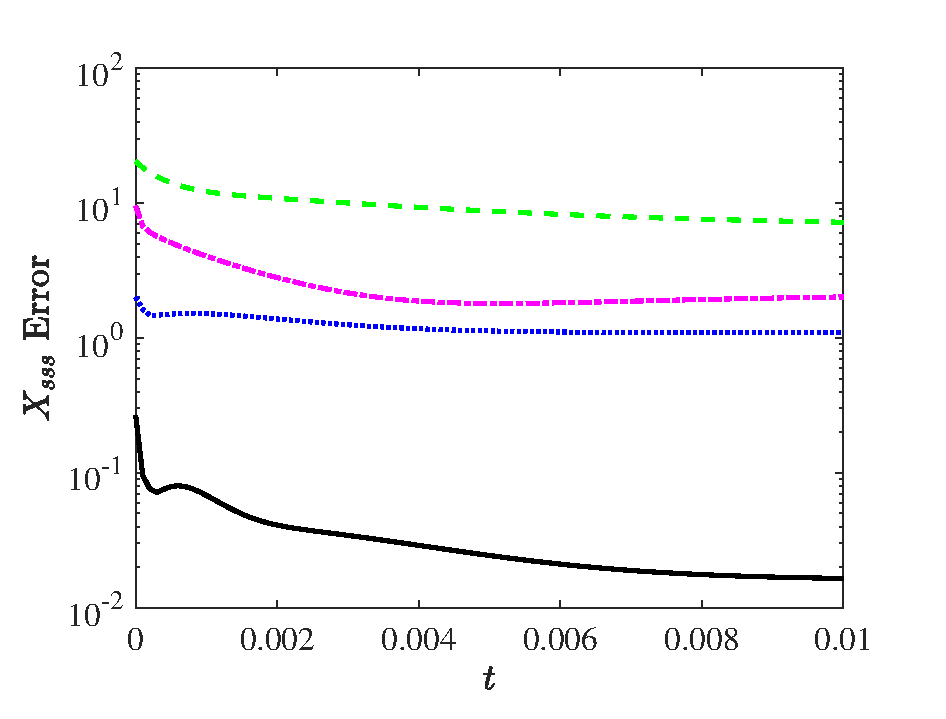
\includegraphics[width=70mm]{BCErrorXsss.eps}}
\caption{Spectral convergence of boundary conditions (a) $\norm{\bm{X}_{ss}(s=0)}_2$, (b) $\norm{\bm{X}_{sss}(s=0)}_2$, both of which should be 0. Shown are solutions for $N=8$ (dashed green), $N=12$ (dashed-dotted pink), $N=16$ (dotted blue), and $N=20$ (solid black), all simulated with RK3 so that the temporal integration is accurate to 10 digits. Values at the boundaries are obtained by differentiation on the $N$ grid, then upsampling to a type 2 grid (that includes the endpoints). }
\label{fig:BCs} 
\end{figure}
